\documentclass[12pt, oneside]{book}
\usepackage[top=0.9in, bottom=0.8in, left=1in, right=0.7in, a4paper]{geometry}
\title{Graph Based Representation of Relational Databases}
\author{Adarsh Mohata, Ajith P S, Ashish Kedia, Sourabh Suman}

 \ifx\pdftexversion\undefined
 \usepackage[dvips]{graphicx}
 \else
 
 \usepackage[pdftex]{graphicx}
 \DeclareGraphicsRule{*}{mps}{*}{}
 \fi
\usepackage{url}
\usepackage{tabularx}
\usepackage{chapterbib}
\usepackage{hyperref}
\usepackage{lscape}
\usepackage{longtable}
\usepackage{float}
\usepackage{url}
\usepackage{amsmath}
\usepackage{multicol}
\usepackage{color}
\usepackage[utf8]{inputenc}
\usepackage{listings}
\usepackage{kbordermatrix}
\usepackage{fancyhdr}
\usepackage{caption}
\usepackage{chngcntr}
\usepackage{pdfpages}
\usepackage{amsmath}
\counterwithin{figure}{chapter}
\counterwithin{table}{chapter}
%\pagestyle{fancy}
\lhead{\leftmark}
\rhead{}
\cfoot{}
\rfoot{\thepage}
\raggedbottom
\renewcommand{\bibname}{References}
\newcommand{\project}{Graph Based Representation of Relational Databases}
\addtocontents{toc}{\protect\setcounter{tocdepth}{1}}

\definecolor{codegreen}{rgb}{0,0.6,0}
\definecolor{codegray}{rgb}{0.5,0.5,0.5}
\definecolor{codepurple}{rgb}{0.58,0,0.82}
\definecolor{backcolour}{rgb}{0.95,0.95,0.92}

\lstdefinestyle{mystyle}
{   language=bash,
    basicstyle=\ttfamily,
    morekeywords={peter@kbpet},
    alsoletter={:~\$},
    morekeywords=[2]{peter@kbpet:},
    keywordstyle=[2]{\color{red}},
    literate={\$}{{\textcolor{red}{\$}}}1 
	    {:}{{\textcolor{red}{:}}}1
	    {~}{{\textcolor{red}{\textasciitilde}}}1,
    backgroundcolor=\color{backcolour},	  
    commentstyle=\color{red},
    keywordstyle=\color{blue},
    numberstyle=\tiny\color{codegray},
    stringstyle=\color{codepurple},
    basicstyle=\footnotesize,
    breakatwhitespace=true,         
    breaklines=true,                 
    captionpos=b,                    
    keepspaces=true,                 
    numbers=left,                    
    numbersep=5pt,                  
    showspaces=false,                
    showstringspaces=false,
    showtabs=false,                  
    tabsize=4
}

\begin{document}
\begin{titlepage}
 \begin{center}
	\emph{A Project Report on} \\
\vspace{1cm}
\large
\textbf{\project} \\
\normalsize
\vspace{5mm}
\emph{Submitted by} \\
\vspace{5mm}
\textbf{Adarsh Mohata - 12IT03 - $VI$ Sem B.Tech} \\
\vspace{1mm}
\textbf{Ajith P S - 12IT04 - $VI$ Sem B.Tech} \\
\vspace{1mm}
\textbf{Ashish Kedia - 12IT14 - $VI$ Sem B.Tech} \\
\vspace{1mm}
\textbf{Sourabh Suman - 12IT82 - $VI$ Sem B.Tech} \\
\vspace{1cm}
\emph{Under the guidance of} \\
\vspace{1cm}
\textbf{Prof. Ananthanarayana V. S.} \\
\textbf{Dept of IT, NITK Surathkal} \\
\vspace{5mm}
\emph{in partial fulfillment for the award of the degree} \\
\vspace{5mm}
\emph{of} \\
\vspace{4mm}
\textbf{Bachelor of Technology} \\
\vspace{4mm}
\emph{in} \\
\vspace{4mm}
\textbf{Information Technology} \\
\vspace{5mm}
\emph{at} \\
\begin{figure}[H]
	\centering
	
\includegraphics[height=3.5cm]{pics/nitk_logo.jpg}
\end{figure}
\vspace{1cm}
\textbf{Department of Information Technology} \\
\vspace{5mm}
\textbf{National Institute of Technology Karnataka, Surathkal} \\
\vspace{5mm}
\text{April 2015}
\end{center}
\end{titlepage}

 \pagebreak \textcolor{white}{text}
\thispagestyle{empty}
\pagenumbering{gobble}
\begin{center}
\Large
\textbf{Department of Information Technology} \\
\normalsize
\textbf{National Institute of Technology Karnataka, Surathkal} \\
\vspace{1cm} \Large
\textbf{Minor Project} \\ \vspace{0.5cm}
\textbf{End Semester Evaluation (April 2015)}
\vspace{1cm}
\end{center}
Course Code : IT 399 \\
Course Title : Minor Project \\
Title of the Project : Graph based storage for Relational Databases \\
Details of Project Group : \\
\vspace{5mm}
\\
\begin{table}[h!]
  \begin{center}
   \begin{tabular}{ p{0.05\textwidth} | p{0.2\textwidth} | p{0.2\textwidth} | p{0.4\textwidth} }
      \hline
      \multicolumn{1}{|c|}{\textbf{S.No}} & \multicolumn{1}{c|}{\textbf{Name}} & \multicolumn{1}{c|}{\textbf{Register No.}} & \multicolumn{1}{c|}{\textbf{Signature with Date}} \\ \hline
      \multicolumn{1}{c}{} & \multicolumn{1}{c}{} & \multicolumn{1}{c}{} & \multicolumn{1}{c}{\hspace{4cm}}\\
      \multicolumn{1}{c}{1} & \multicolumn{1}{c}{Adarsh Mohata} & \multicolumn{1}{c}{12IT03} & \multicolumn{1}{c}{}\\
      \multicolumn{1}{c}{} & \multicolumn{1}{c}{} & \multicolumn{1}{c}{} & \multicolumn{1}{c}{}\\
      \multicolumn{1}{c}{2} & \multicolumn{1}{c}{Ajith P S} & \multicolumn{1}{c}{12IT04} & \multicolumn{1}{c}{}\\
      \multicolumn{1}{c}{} & \multicolumn{1}{c}{} & \multicolumn{1}{c}{} & \multicolumn{1}{c}{}\\
      \multicolumn{1}{c}{3} & \multicolumn{1}{c}{Ashish Kedia} & \multicolumn{1}{c}{12IT14} & \multicolumn{1}{c}{}\\
      \multicolumn{1}{c}{} & \multicolumn{1}{c}{} & \multicolumn{1}{c}{} & \multicolumn{1}{c}{}\\
      \multicolumn{1}{c}{4} & \multicolumn{1}{c}{Sourabh Suman} & \multicolumn{1}{c}{12IT82} & \multicolumn{1}{c}{}\\
      \multicolumn{1}{c}{} & \multicolumn{1}{c}{} & \multicolumn{1}{c}{} & \multicolumn{1}{c}{}\\
   \end{tabular}

  \end{center}

\end{table}
\\
\\
\begin{tabular}{l@{\hskip 4cm} r}
	\line(1,0){150} \\
	 Prof. Ananthanarayana V. S. \\
	 Dept. of IT, NITK \\
	 Project Mentor \\ 
\end{tabular}

\vspace{4cm}
\begin{flushleft}
Place: NITK Surathkal, Mangalore \\
Date: \today
\end{flushleft}

\pagebreak \textcolor{white}{text}
\thispagestyle{empty}
\begin{center}
	\textbf{ \huge Abstract}
\end{center}
\vspace{1cm}
Relational Database Management Systems has been there for quite a few decades. They are still the most popular means of storing huge amount of data on disk. Relational databases are efficient in most cases, however in certain types of queries (Join) they fail to compute the result efficiently. In recent times, quite a bit of research has been done on Graph Databases - which seems like  a promising solution to the bottleneck. Many implementation of such databases have come up - Google's Cayley, Neo4j, etc. However even these graph databases suffer from several overheads.
\par
This project aims at exploring the various ways of using a graph-like storage model for traditional Relational Databases and optimize it to perform Inner Join and Aggregate Queries efficiently.
\par
\textbf{Keywords : }Database, Graph, Relational

\thispagestyle{empty}
{\listoffigures}
{\listoftables}
{\tableofcontents}

\setcounter{page}{1}
\pagenumbering{arabic}

\chapter{Introduction}
In the world of computer science, a graph database is a database that uses graph structures for semantic queries with nodes, edges, and properties to represent and store data. A graph database is any storage system that provides index-free adjacency. This means that every element contains a direct pointer to its adjacent elements and no index lookups are necessary. Graph Databases is being extensively researched upon in recent years. There are are several implementation of graph databases available like Neo4j \cite{neo4j}, Titan \cite{titan} and OrientDB \cite{orientdb} all of which is based the same principle.
\begin{figure}[h]
 \begin{center}
  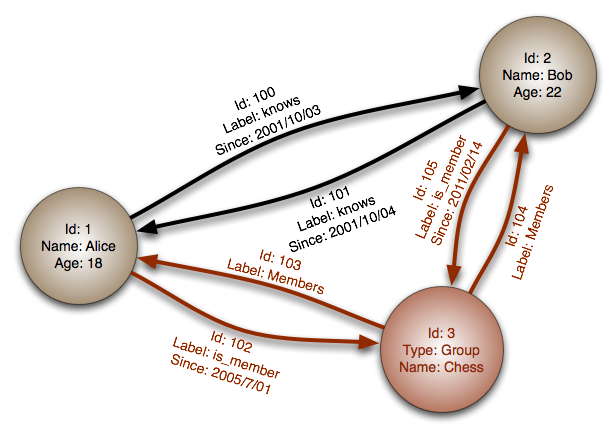
\includegraphics[width=0.7\textwidth]{pics/graph.png}
  \caption{A Graph Database}
 \end{center}
\end{figure}
\section{Motivation}
Graph Databases seems like a promising model to solve all the problems that exist with the current relational databases. They provide an optimal way to compute the equivalent of the join query in a relational database. They can also scale very well and can handle large volume of data. Several Load Balancing Techniques can also be used to optimize queries during large scale Graph Processing \cite{load_balancing}. Because of these reasons Graph Database is being widely used. Angles et. al have surveyed the most popular graph based model \cite{graph_database_survey}. \\ \par
However, Graph databases have their own overheads and drawbacks. Sometimes it is very difficult or even impossible to construct the equivalent relational database from a graph database. Moreover, graph databases don't use SQL and as such it is very difficult for the programmers to realize the query they want to perform. Even if the developers are able to realize the query, the existing queries in the system has to be changed which will take a lot of resources. Organizations which have made huge investments on their database system might not be willing to switch to graph databases. Vicknair et. al have drawn a good comparison between graph based databases and traditional relational databases in terms of performance and storage requirements \cite{graph_relational_comparison}. \\ \par
Owing to these reasons, the use of graph database is currently limited. We were motivated to resolve this problem by taking a middle path between graph and relational databases. We wanted to explore the various ways to optimize the query execution time as well as the storage of the currently popular relational databases. We also wanted to eliminate all the redundancy in a typical relational database.

\section{Problem Description}
In this project we concentrate on 2 major problems of relational database - the data redundancy and expensive join queries.
\subsection{Data Redundancy}
To demonstrate this problem let us consider a typical Employee table in a relational database ~\ref{tab:employee_demo}. Each Employee record has all the typical attributes associated with it like \emph{id} (primary or identifying attribute), \emph{name}, \emph{department}, \emph{salary}, etc. 
\begin{table}[h]
\begin{center}
    \begin{tabular}{| m{0.01\textwidth} | m{0.05\textwidth} | m{0.15\textwidth} | m{0.01\textwidth} | m{0.01\textwidth} | m{0.01\textwidth} | m{0.01\textwidth} | @{}m{0pt}@{}}
    \hline
    \multicolumn{1}{|c|}{} & \multicolumn{1}{c|}{} & \multicolumn{1}{c|}{} & \multicolumn{1}{c|}{} & \multicolumn{1}{c|}{} & \multicolumn{1}{c|}{} & \multicolumn{1}{c|}{} &  \\
    \multicolumn{1}{|c|}{\textbf{Id}} & \multicolumn{1}{c|}{\textbf{Name}} & \multicolumn{1}{c|}{\textbf{Department}} & \multicolumn{1}{c|}{\textbf{Age}} & \multicolumn{1}{c|}{\textbf{Product}} & \multicolumn{1}{c|}{\textbf{Location}} & \multicolumn{1}{c|}{\textbf{Salary}} & \\
    \multicolumn{1}{|c|}{} & \multicolumn{1}{c|}{} & \multicolumn{1}{c|}{} & \multicolumn{1}{c|}{} & \multicolumn{1}{c|}{} & \multicolumn{1}{c|}{} & \multicolumn{1}{c|}{} &  \\
    \hline
    1 & John & Information Technology & 40 & Firefox & Mumbai & 20000 & \\ [1ex] \hline
    2 & David & Information Technology & 42 & Firefox & Mumbai & 23000 & \\ [1ex] \hline
    3 & Roger & Information Technology & 34 & Firefox & Mumbai & 25000 & \\ [1ex] \hline
    4 & Paul & Information Technology & 27 & Firefox & Mumbai & 20000 & \\ [1ex] \hline
    5 & James & Information Technology & 45 & Firefox & Mumbai & 20000 & \\ [1ex] \hline
    6 & Charlie & Information Technology & 40 & Firefox & Mumbai & 25000 & \\ [1ex] \hline
    7 & Shaun & Information Technology & 40 & Firefox & Mumbai & 25000 & \\ [1ex] \hline
    8 & Jade & Information Technology & 24 & Firefox & Mumbai & 25000 & \\ [1ex] \hline
    9 & Jack & Information Technology & 34 & Firefox & Mumbai & 23000 & \\ [1ex] \hline
    \end{tabular}
\end{center}
    \caption{A sample Employee Table with redundant data}
    \label{tab:employee_demo}
\end{table}
As we can observe that each department is uniquely associated with a product and is located in a particular city. The same triplet of values - Information Technology, Firefox and Mumbai - is stored for each of the 9 employees working with that product. This wastes a lot of space. This type of redundancy is known an strong redundancy \cite{redundancy}. It is caused when the table is in a de-normalized state. The traditional way to reduce such redundancy is to decompose this table into multiple tables. One way in which this table can be decomposed in demonstrated in table ~\ref{tab:emp_normal} and table ~\ref{tab:product}. The product details is stored in a separate table and the Employee table refers to the product table as foreign key.

\begin{table}
    \centering
    \begin{tabular}{| c | c | c | c | c | @{}m{0pt}@{}}
    \hline
    \multicolumn{1}{|c|}{} & \multicolumn{1}{c|}{} & \multicolumn{1}{c|}{} & \multicolumn{1}{c|}{} & \multicolumn{1}{c|}{} &  \\
    \multicolumn{1}{|c|}{\textbf{Id}} & \multicolumn{1}{c|}{\textbf{Name}} & \multicolumn{1}{c|}{\textbf{Age}} & \multicolumn{1}{c|}{\textbf{Pr. ID}} & \multicolumn{1}{c|}{\textbf{Salary}} & \\
    \multicolumn{1}{|c|}{} & \multicolumn{1}{c|}{} & \multicolumn{1}{c|}{} & \multicolumn{1}{c|}{} & \multicolumn{1}{c|}{} &  \\
    \hline
    1 & John & 40 & 1 & 20000 & \\ [1ex] \hline
    2 & David & 42 & 1 & 23000 & \\ [1ex] \hline
    3 & Roger & 34 & 1 & 25000 & \\ [1ex] \hline
    4 & Paul & 27 & 1 & 20000 & \\ [1ex] \hline
    5 & James & 45 & 1 & 20000 & \\ [1ex] \hline
    6 & Charlie & 40 & 1 & 25000 & \\ [1ex] \hline
    7 & Shaun & 40 & 1 & 25000 & \\ [1ex] \hline
    8 & Jade & 24 & 1 & 25000 & \\ [1ex] \hline
    9 & Jack & 34 & 1 & 23000 & \\ [1ex] \hline
    \end{tabular}
    \caption{A normalized Employee Table}
    \label{tab:emp_normal}
\end{table}

\begin{table}
    \centering
    \begin{tabular}{| c | c | c | c | @{}m{0pt}@{}}
    \hline
    \multicolumn{1}{|c|}{} & \multicolumn{1}{c|}{} & \multicolumn{1}{c|}{} & \multicolumn{1}{c|}{} &  \\
    \multicolumn{1}{|c|}{\textbf{Id}} & \multicolumn{1}{c|}{\textbf{Department}} & \multicolumn{1}{c|}{\textbf{Product}} & \multicolumn{1}{c|}{\textbf{Location}} & \\
    \multicolumn{1}{|c|}{} & \multicolumn{1}{c|}{} & \multicolumn{1}{c|}{} & \multicolumn{1}{c|}{} &  \\
    \hline
    1 & Information Technology & Firefox & Mumbai & \\ [1ex] \hline
    \end{tabular}
    \caption{A sample product table}
    \label{tab:product}
\end{table}
There may be redundancy in a single attribute column also - like Salary. The Salary can only take one of 3 values - \{20000, 23000, 25000\}. These values are repeated. This type of redundancy is known as weak redundancy. Even this can be decomposed into multiple tables and linked via foreign key. However, Normalization of tables have a overhead - an expensive join query has to be performed in order to obtain the original table. To perform a join operation, a relational database management system will take the Cartesian Product of the two tables. This has been discussed in detail in section ~\ref{sec:join}. \par
We have tried to reduce this data redundancy by modeling each unique value as a separate node in a graph and all the records that has this value only stores a pointer to the actual node which stores the value. The value is stored only once in the memory and a pointer is added to that same value whenever a new record with that value is inserted. This optimizes storage requirements (especially if the value is large compared to size of a pointer). This also helps achieve data consistency. If the value is changed for some reason, all the records pointing to it automatically changes.
\subsection{Expensive Join Queries}
\label{sec:join}
Often user has to fetch data spanning across multiple tables in a database. This is achieved using Join Queries. User specifies the tables from which the records have to be selected. Typically user also specifies the join condition i.e., how the two tables are related. For Example, the Employee and Product Tables are joined based on the fact that the \emph{Pr.ID} attribute in Employee table corresponds to the \emph{Id} attribute in product table and thus must be equal. This is an Inner Join. Join Queries are common in applications using relational database to store data. Theoretically, the time complexity of each Join Operation is $\mathcal{O}\left( mn \right)$ where, $m, n$ is the number of records in the two tables respectively. This is inefficient considering the frequency of join operations. We have tried to optimize the inner join operation. Our graph based storage can theoretically perform an inner join in linear time. 

\chapter{Literature Review}
Relational Databases are a common choice for primary data storage structure in both academic and commercial pursuits since the 1970s. The Relational Model organizes data into one or more tables of rows and columns, with a unique key for each tuple. Generally, each entity type described in a database has its own table, the tuples representing instances of that entity and the columns representing the attribute values describing each instance. They provide relational operators to manipulate the data in tabular form. Most of the relational databases use SQL as their query language. Relational database systems are generally efficient unless the data contains many relationships requiring joins of large tables. These costly join operations are usually addressed by denormalizing data to reduce the number of joins necessary.  
\section{Graph Model}
In recent years, software developers have been investigating storage alternatives to relational databases. BigTable, Cassandra, CouchDB, Project Voldemort, and Dynamo are all NoSQL projects, as they are all high-volume data stores that actively reject the relational model. In the graph model, nodes represent entities. Properties are pertinent information that relate to nodes. Edges are the lines that connect nodes to nodes or nodes to properties and they represent the relationship between the two. Compared with relational databases, graph databases are often faster for associative data sets and map more directly to the structure of object-oriented applications \cite{object_graph}. Graph based databases can scale more naturally to large data sets as they do not typically require expensive join operations. As they depend less on a rigid schema, they are more suitable to manage ad hoc and changing data with evolving schema. Graph databases are a powerful tool for graph-like queries, for example computing the shortest path between two nodes in the graph.\\
\par
However, relational databases are typically faster at performing the same operation on large numbers of data elements. A relational database is much faster when operating on huge numbers of records. In a graph database, each record has to be examined individually during a query in order to determine the structure of the data, while this is known ahead of time in a relational database. Relational databases use less storage space, because they don't have to store all of those relationships.

\section{Problem Statement}
To develop a data management system based on graph structure in order to optimize the query execution time especially join and aggregate queries and eliminate data redundancy in a relational model to some extent while retaining other advantages of relational database system in terms of performance of other queries.  

\section{Research Objectives}
\begin{itemize}
 \item To compare the relational model with the existing graph models.
 \item To develop a model which can represent relational database.
 \item To define relational algebraic operations on the model such that it has most of the advantages of both the models.
 \item To understand the differences of the proposed model with the graph model.
 \item To realize the limitations of the proposed model.
\end{itemize}

\chapter{Methodology}
In this chapter we will discuss our proposed model in detail. We will describe how the data is handled and manipulated.
Relational database performs inefficiently in a join type query. Graph database is able to perform join type queries quite fast because it stores the data using a graph structure. But because of the model used, it is sometimes unable to represent all kinds of relational databases. Realizing that the problem lies with the model of the graph used, we came up with our own model to represent relational databases, using graphs.\\ \par
\section{Definitions}
A single relation(table) can be represented a set of nodes and edges in our proposed graph storage, Before we discuss the model in detail, we define certain terminology used in the context of this project.
\begin{enumerate}
 \item \textbf{Domain} - Each attribute of a relation is a domain in our model. For Example, for an employee table, the relevant domains are \emph{Name}, \emph{Salary}, \emph{Age}, etc. Unlike traditional relational databases two relation can share same domain i.e., a domain can belong to multiple tables. For example, in Employee-Product example (\ref{tab:employee_demo}) \emph{Pr.Id} belongs to both Employee table and Product table. Each table can have separate attribute names for the domain. A domain is nothing but a list of unique Attribute Nodes.
 \item \textbf{Attribute Node} - Attribute Node is a graph node which contains actual data. Each Attribute Node contains only one value. An attribute node also has a list of pointers to the records that have its stored value in corresponding domain.
 \item \textbf{Main Node} - Each main node represents a record in the table. Main node do not contain values - rather they point to $n$ different attribute nodes (one each in $n$ domains) where $n$ is the number of attributes. Main Node of a table may also point to the main node of any other table in case of foreign key i.e., parent-child relationship.
\end{enumerate}

\section{Overall Structure}
A database consists of multiple tables. Each table is a collection of domains (one domain corresponding to each attribute) and a list of main node records. Each Domain is a collection of attribute nodes. Each attribute node contains the actual data elements. Nodes are connected to each other by edges (using pointers). A brief overview of the model has been illustrated in figure ~\ref{fig:overview}
\begin{figure}[t]
 \centering
 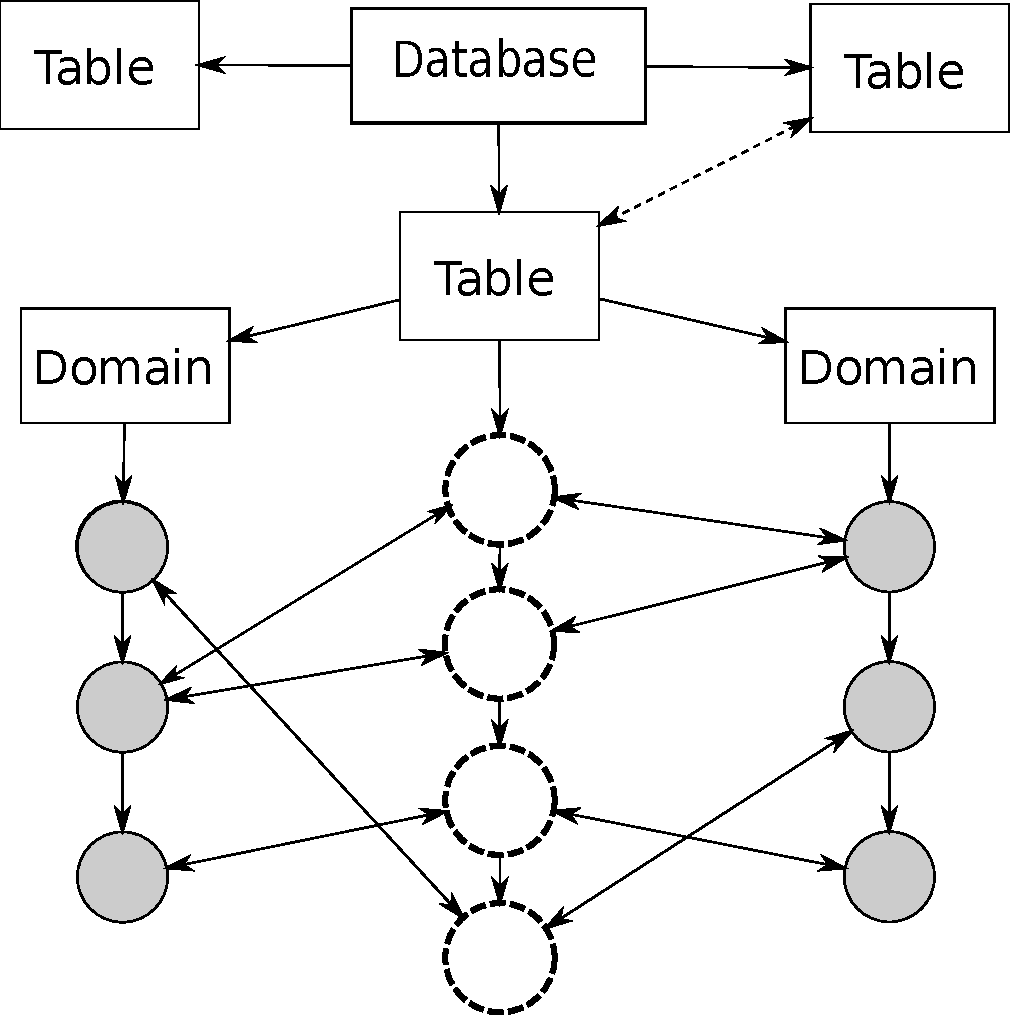
\includegraphics[width=0.8\textwidth]{pics/model.pdf}
 \caption{Overview of Proposed Model}
 \label{fig:overview}
\end{figure}

\section{Constraints}
In this section, we will discuss about the constraints that are added to the relations in a traditional RDBMS to ensure data integrity and logical consistency.
\subsection{Primary Key}
In a Relational Database, Primary Key is a collection of one or more attributes of a relation which uniquely identifies a tuple i.e., each record will have a different value of primary key. The main thing to note here is that Primary Key can span over multiple attributes i.e., a collection of attributes together may uniquely identify a primary key. While performing an insertion operation, it is essential to check that no previous record has the same value for the primary key. When primary key spans over multiple attributes (or domains in our proposed model) one has to check if the combination of values being inserted is unique. The primary key constraint has been illustrated in figure ~\ref{fig:primary_key}. A record (in a relation storing data about engineering institutes) is uniquely determined by combination of department and institute.
\begin{figure}
 \centering
 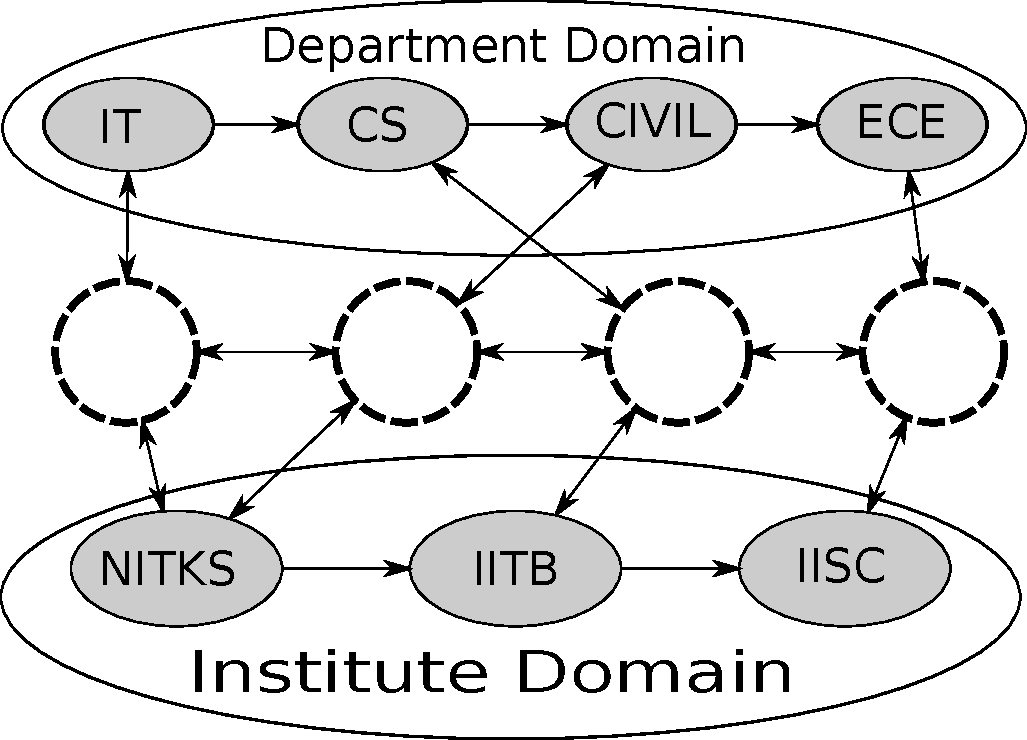
\includegraphics[width=0.8\textwidth]{pics/primary_key.pdf}
 \caption{Primary Keys in Proposed Model}
 \label{fig:primary_key}
\end{figure}

\subsection{Foreign Key}
When multiple relations are involved with some of them having foreign key relation, then our proposed model is extended to accommodate those constraints. Storage of foreign key in our proposed model has been illustrated in figure ~\ref{fig:foreign_key}.
\begin{figure}[h]
 \centering
 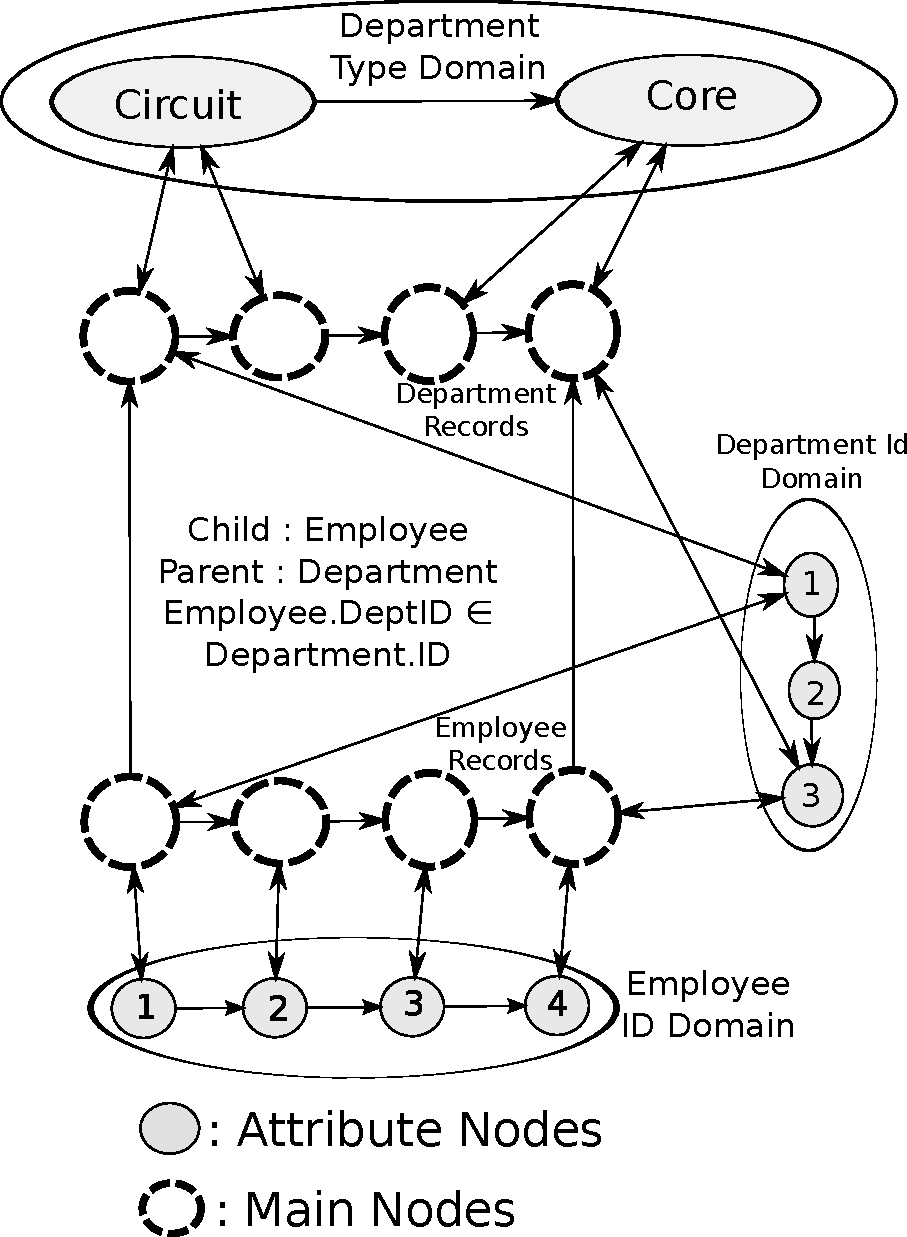
\includegraphics[width=0.6\textwidth]{pics/foreign_key.pdf}
 \caption{Handling of Foreign Key Constraints}
 \label{fig:foreign_key}
\end{figure}
Major points to observe are as follows :
\begin{itemize}
 \item Suppose relation A has a foreign key relationship with relation B. Then relation A is said to be the child and relation B is said to be the parent relation.
 \item Each tuple (modeled as Main Node) in the child relation will refer to a single tuple in the parent relation.
 \item Multiple tuples in child relation can refer to the same tuple in the parent relation.
 \item The attribute in which foreign key constraint is applied is shared between the child relation and parent relation i.e., a single domain is shared between 2
 tables.
 \item A child relation will always refer to the primary key in the parent relation. Thus, if the primary key in parent relation spans over multiple domains, the foreign key in child relation also spans over multiple domains and each domain is shared between parent and child.
 \item A relation can have multiple foreign key constraint each referring to a different relation in the database.
\end{itemize}
There are 3 other ways in which the foreign key constraint can be handled. We came up with these methods during our research however we chose to implement the model that has been described above. The methods are described as follows :
\begin{enumerate}
 \item \textbf{Direct Connection Model} - Each Domain will belong to a single table. Whenever a child refers to the parent table, only the main node of record in the child relation is bidirectionally connected to the main node of the corresponding record in parent relation. Further the meta-data about the foreign key is stored separately in database. This model requires 2 edges between each foreign key connection and it is very efficient when corresponding tuples in child relation are to be fetched given a tuple in parent relation. However, queries which involves accessing the attribute nodes of the foreign key domain will be expensive as the only path between the shared domain's attribute nodes and main nodes of child relation is via parent table.
 \item \textbf{Shared Domain Model} - There is no direct connection between child and parent main nodes. In this case, a domain can belong to multiple tables and a domain is bidirectionally connected to both the parent and child relation. Attribute nodes of the shared domain is also bi-directionally connected with multiple tuples in child relation and a single tuple in parent relation. This model requires 4 edges for each foreign key connection. Here aggregate queries on child relation can be performed faster as the shared domain is directly accessible to both the child and the parent relation. However, accessing corresponding parent relation's record given a child relation's record or vice-versa is expensive.
 \item \textbf{Duplicate Domain Model} - There are two copies of the shared domain - one belonging to each child and parent relation. And a unidirectional (or bidirectional if need be) edge between tuples in the child relation and tuples in the parent relation exist. This model requires 2 or 3 edges as well as an attribute node for each foreign key connection. This model has a lot of storage overhead but it allows all the operation to be performed in the most optimal fashion. However, due to data replication, this model may cause data inconsistency.
\end{enumerate}

\section{Records and their Attributes}
In this section we will discuss how a record and its associated values are stored in our proposed graph storage model.
\subsection{Tuple of a Relation - Main Node}
\label{sec:tuple}
We propose use of linked list to store all the main nodes. The nature of linked linked can be unidirectional (singly) or bidirectional (doubly). A singly linked list or a vector of main nodes will have less storage overhead, however the delete operation might be expensive. A possible workaround of this problem is to store a boolean field with each main node which marks the tuple as well as the associated values in the attribute nodes as invalid. After a regular interval the whole list can be traversed and all the marked records can be deleted. This way we save on space. However, whenever brute force method is used to execute the select query an extra data-access is required to check if the data is valid or not.
\subsection{Attributes of Record}
Each column in a table of a relational database has its own domain and it contains a list of values. The list may be singly linked list or doubly linked list depending on the requirement. The same argument as section ~\ref{sec:tuple} applies here. Each node which contains the actual record is not of fixed size. Size of an attribute node is dynamic - it depends on size of the value unlike traditional relational databases where the size of an attribute is fixed and specified at the time of creating table. An attribute node will be bidirectionally connected with all the main nodes in all the tables (in case of shared domains) that contains this value. This means aggregate queries can be performed much faster. As an example, let us assume that in a relation containing 50,000 records about the employees of an organization, we intend to find all employees with a given salary say \$100. Now, let us assume that there are only 10 such employees. Then we can find all those 10 tuples with at max 10 record access in worst case i.e., $\mathcal{O}(k)$, where $k = 10$ is the size of the result. In traditional databases if there is no indexing on the salary attribute then the same query may take $\mathcal{O}(n)$, where $n = 50000$ is the number of records in the table.

\chapter{Work Done}
As of now, we have been able to implement a basic version of the proposed graph like storage model which supports all the queries of a traditional relational database. The whole graph storage model has been implemented using C\verb!++!. We chose to go with C\verb!++! owing to its speed, object oriented nature and the powerful Standard Template Library. STL containers like \emph{vectors}, \emph{string} and \emph{set} are used throughout the source code. We have also used methods provided by STL to handle data. The user input is taken via standard input stream i.e., command line. Similarly all output is printed on standard output stream. No GUI has been provided as of now. All data is stored in main memory.
\section{Implementation}
We have implemented the following core functionalities which the user can choose from the main menu :
\begin{multicols}{2}
 \begin{itemize}
  \item Creating Tables
  \item Describing Existing Table
  \item Inserting Records in table
  \item Printing Table
  \item Indexing Records
  \item Selecting from single table
  \item Deleting Records in table
  \item Updating Records in table
  \item Joining two Tables
  \item Clearing Memory Allocated
 \end{itemize}
\end{multicols}

\subsection{Indexing}
Trie is the optimal indexing methodology that maps a string to its corresponding node in the graph. The algorithmic complexity of inserting and querying a string in trie is $\mathcal{O} \left( d\right)$ where, $d$ is the length of the string mapped. The data structure can be further optimized in terms of storage requirements by using a compressed trie or a Radix tree. The \emph{trie} data structure has been illustrated in figure ~\ref{fig:trie}.
\begin{figure}
 \centering
 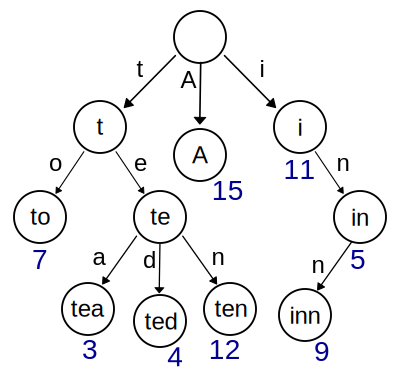
\includegraphics[width=0.5\textwidth]{pics/trie.pdf}
 \caption{Trie Data Structure for Indexing}
 \label{fig:trie}
\end{figure}

The \emph{trie} class in the source code provides all the properties and functions required to index string data. The trie also has a composite class called \emph{trie\_node} associated with it which represents a node in the trie and stores a single character of the string. Each node in trie contains edges to the 256 possible nodes in the next level. Each domain has it's own trie. The \emph{trie} class provides 2 major methods :
\begin{itemize}
 \item \textbf{Value Look Up} - to lookup a string value and get the attribute node which stores this value in the domain
 \item \textbf{Insert Value} - index a new string value along with the attribute node which stores the value being inserted
\end{itemize}

\subsection{Code Structure}
The Code is divided into multiple files for ease of development. Each file provides one or more classes that are a logical entity. The details have been discussed in the following section :
\begin{enumerate}
 \item \textbf{Database} - The database class is the root class that contains all the data. It only contains a list of all the tables. Currently the system supports only one database. It provides functionalities to add a new table, compute the size of all tables and delete all the tables on demand.
 \item \textbf{Table} - The table class represents a relation. This class provides most of the functionalities of the system. It provides all the table related functionalities like measuring size, insertion, selection, projection, update, delete etc. It also provides a function to delete the table on demand. The table class has been divided into 2 files namely - \emph{table.h} and \emph{select.h}. A few utility functionalities like comparing 2 values given a data type, traversing records from parent relation to child relation or vice-versa. A few wrapper type utility classes like \emph{value\_expression} are also provided which helps in passing around a bunch of logically related set of values from one function to another. Table class stores several meta data about the relation and also provides methods to access or manipulate those meta-data. These meta-data include primary key associated with the relation, foreign key constraints and edges to respective domains. Useful methods associated with these meta data are adding primary key, checking existence of record with a given primary key, fetching all records in child relation, fetching record from parent relation, etc. Overall the \emph{table} class provides various independent modules of code in form of functions which are used throughout the database.
 \item \textbf{Main Node} - This class represents a typical tuple in a table. Although no data is stored in Main Node but it points to the corresponding attribute nodes. A Linked List of main nodes makes up a Table. Main node only has a vector of pointers to the corresponding attribute nodes. Each main node belonging to the same table points to same number of attributes. The main node class also provides functionalities to access / update a particular value in that tuple.
 \item \textbf{Domain} - It represents the domain of a data. It is a linked list of all the valid values that an attribute can take. It provides functionality like searching, adding and deleting attribute nodes. It also provides function to measure storage requirements. Since a domain can belong to multiple tables, a domain also stores meta-data about the different tables it belongs to. The most important functionality provided by the \emph{domain} class is to retrieve a list of all the main nodes connected with the attribute node of a given value.
 \item \textbf{Attribute Node} - It is the smallest logical entity that stores the actual data. Only one copy of a particular value is stored in a domain to avoid redundancy. It also stores a list of pointers to all the records (in all the tables) that are pointing to it.
 \item \textbf{Testing} - The file \emph{test.h} provides methods to create a sample database. It creates multiple tables and inserts thousands of records in each table. It also measures metrics such as \emph{time} and \emph{space} required to perform those insertion operations. A vigorous testing was performed in order to ensure that the system was stable and that there were no memory leaks. Our implementation is only limited by the main memory available on the system running the database server.
\end{enumerate}

\section{Results and Analysis}
The Results of our study can be divided into two sections - Storage and Time. We have performed both theoretical as well as practical memory bound calculations. \\
\subsection{Theoretical Calculations}
Each of the record in the proposed graph based storage has following extra data :
\begin{itemize}
 \item Pointer from Main Node to each Attribute Node
 \item Pointer from each Attribute Node to Main Node
 \item Pointer from one Attribute data to the next Attribute data (Next Pointer of linked list)
 \item Pointer from one main node to next main node in the table (Next Pointer of the Linked List)
\end{itemize}
Thus the size occupied by a table in the graph model can be equated using the following equation :
\begin{equation}
  Size\_Graph = (n \times x \times (rs + (attr \times ptr)) ) + (n \times ptr \times (2 \times attr + 1))
  \label{grsize}
\end{equation}
where, \\
$Size\_Graph$ = Size occupied by Graph Storage Engine, \\
$x$ = Fraction of tuples that are unique, \\
$rs$ = Theoretical size of each tuple in a table, \\
$n$ = Number of records in a table, \\
$attr$ = Number of Attributes in the table, \\
$ptr$ = Size of a pointer variable \\

The above equation illustrates the growth of database on the proposed graph storage engine. For a traditional Relational Database the space occupied by the data in the memory can be arrived at using the following equations :
\begin{equation}
 Size\_RDBMS = n \times rs
 \label{rdbmssize}
\end{equation}
where, \\
$Size\_RDBMS$ = Size occupied by the Relational Database Engine, \\
$n$ = Number of tuples in a table, \\
$rs$ = Theoretical size of each tuple in a table \\

\par
Using equation ~\ref{grsize} and ~\ref{rdbmssize} we can conclude that given a particular table (Fixed number of attributes) on a particular system (Fixed Pointer Size) the Space complexity of both the engines is same i.e., $\mathcal{O}\left( n\right)$ where, $n$ is the number of tuples in the table. However, for absolute measurement we can equate the two equation to obtain a break-even point after which the graph storage engine is more efficient than the traditional relational model.
\begin{center}
  \begin{math}
    (n \times x \times (rs + (attr \times ptr)) ) + (n \times ptr \times (2 \times attr + 1 )) < n \times rs
  \end{math}\\
  \begin{math}
    ( x \times ( rs + ( attr \times ptr ) ) ) + ( ptr \times (2 \times attr + 1 )) < rs
  \end{math}
\end{center}
\[
 x  < \frac{ rs - ( ptr \times (2 \times attr + 1 )) }{rs + ( attr \times ptr )}
\]

Assuming a typical record size to be 400 bytes, number of attributes to be 5, pointer size to be 8 bytes (x64 systems) we get,
\[
 x < \frac{400 - (8 \times (2 \times 5 + 1))}{400 + (5 \times 8)}
\]
\[
 x < \frac{400 - (88)}{400 + 40} = \frac{312}{440} \sim 0.71
\]
which means that if at-least 29\% of values in a table are repeated then the graph storage engine occupies less space than the relational databases. In a real-life database there are numerous duplicate entries and thus the proposed storage model may perform better.

\subsection{Testing Environment}
The machine on which the testing was performed and results were observed had the following configuration :
\begin{itemize}
 \item \textbf{OS} - Linux (Debian - Ubuntu 14.04)
 \item \textbf{Processor} - Intel 3rd Gen i5 Quad Core
 \item \textbf{Main Memory} - 4 GB
 \item \textbf{Architecture} - 32 bit
 \item \textbf{Compiler Used} - g\verb!++!
\end{itemize}
The test data that we generated had the following structure and characteristics :
\begin{itemize}
\item \textbf{Number of Database} - 1
 \item \textbf{Number of Tables} - Two
 \item \textbf{Number of Attributes in Employee} - 6 (ID, Name, Address, Salary, Sex, Dept\_ID)
 \item \textbf{Type of Attribute} - Integer (Primary key), String (1-30), String (1-50), Float, String(4, 6), Integer (Foreign Key)
 \item \textbf{Redundancy of Values} - 40 \%
\end{itemize}
The Maximum length of string data type was specified and a random length was used for each record. Random Records were generated using the psuedorandom generators provided by the standard C Library.

\subsection{Practical Observation of Size}
\begin{figure}[ht]
  \centering
   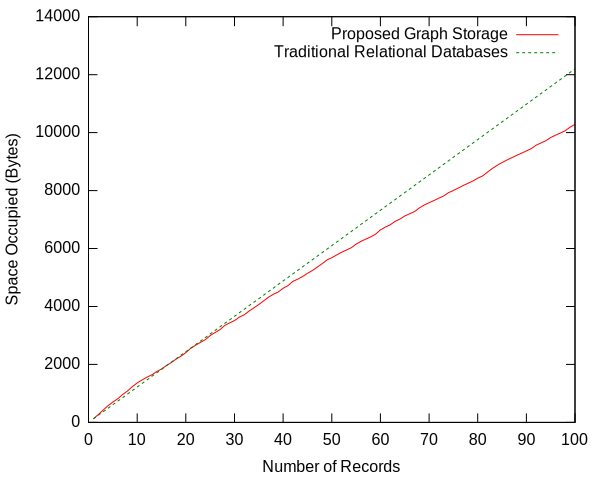
\includegraphics[width=\textwidth]{pics/100.pdf}
   \caption{Comparison of Size of 100 records}
   \label{fig:100result}
\end{figure}
We created an equivalent table in both traditional Relational DBMS and our model. We measured the size occupied by both the models. We have plotted several graphs. Numbers of records are increasing along X axis, while space occupied by the model is increasing along Y axis.
\begin{enumerate}
 \item \textbf{100 Records} - Number of records was varied between 1 to 100. Observations were made after every record. The graph obtained is shown in figure ~\ref{fig:100result}
  \item \textbf{1000 Records} - Number of records was varied between 1 to 1000. Observations were made after every 10 record. The graph obtained is shown in figure ~\ref{fig:1000result}
 \begin{figure}[H]
  \begin{center}
   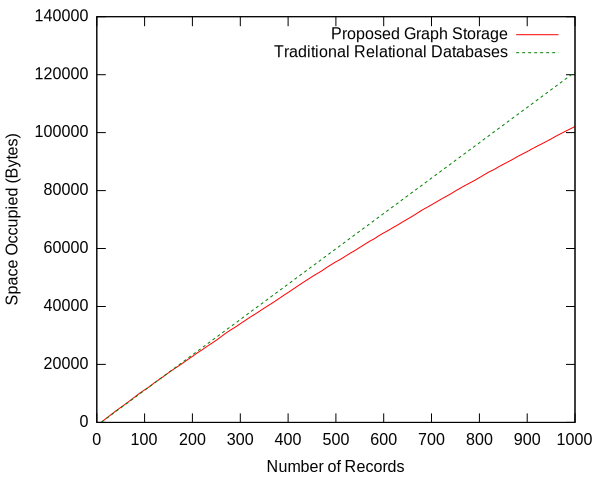
\includegraphics[width=\textwidth]{pics/1000.pdf}[H]
   \caption{Comparison of Size of 1000 records}
   \label{fig:1000result}
  \end{center}
 \end{figure}
  \item \textbf{10000 Records} - Number of records was varied from 1 to 10000. Observations were made after every 100 record. The graph obtained is shown in figure ~\ref{fig:10000result}
 \begin{figure}[H]
  \begin{center}
   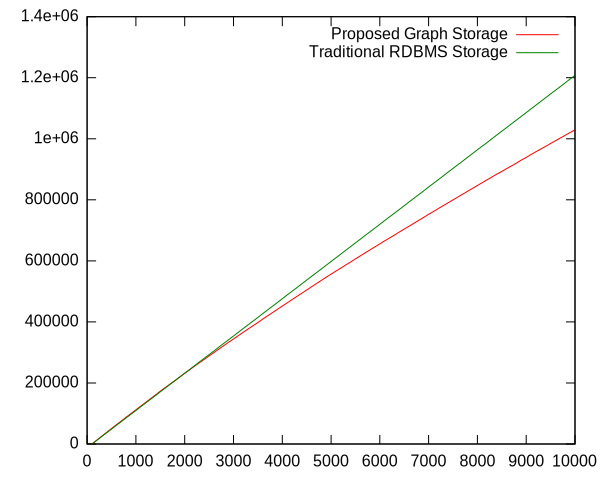
\includegraphics[width=\textwidth]{pics/10000.pdf}
   \caption{Comparison of Size of 10000 records}
   \label{fig:10000result}
  \end{center}
 \end{figure}
 \item \textbf{90000 Records} - Number of records was varied from 1 to 90000. Observations were made after every 900 record. The graph obtained is shown in figure ~\ref{fig:90000result}
 \begin{figure}[ht]
  \begin{center}
   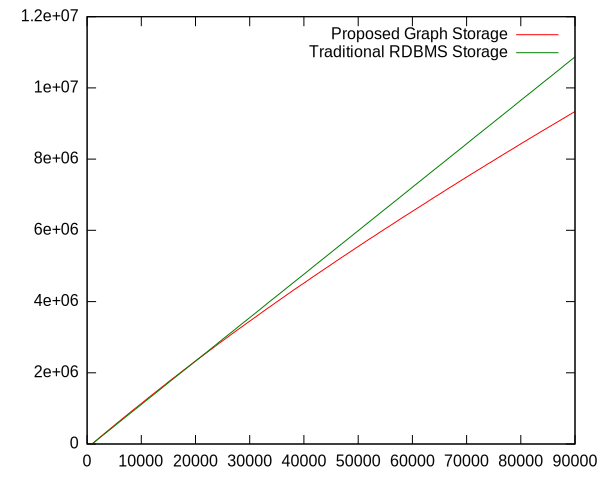
\includegraphics[width=\textwidth]{pics/90000.pdf}
   \caption{Comparison of Size of 90000 records}
   \label{fig:90000result}
  \end{center}
 \end{figure}
\end{enumerate}
\par
It is clearly evident from these plots that traditional RDBMS increases their storage linearly. Our proposed model also scales linearly. The initial size occupied by our proposed model is more but the slope of our model is smaller than that of relational database storage. In the long run, our graph based model performs better. \par
However, several factors were not accounted while making these observations - which makes these observations a little less reliable. Owing to limitations of the physical resources available with us, we were unable to test the system for larger dataset. We intend to perform a more vigorous analysis of the storage requirement in future.
\subsection{Practical Observation of Time}
We chose to measure the time taken to execute the most expensive query - Join. The exact query that we executed was : \\
\begin{center}
 \textbf{Select $*$ from employee, department where employee.id $>$ 10 AND \\
 department.id $<$ 50 AND employee.dept\_id = department.id}
\end{center}
We measured the time taken with different number of records in the child relation i.e., Employee relation. The number of records in the parent relation (Department) was kept constant i.e, 100. The points of observation in child relation were - 100, 1000, 10000, 20000, 40000, 60000, 80000 and 90000. The results have been illustrated in figure ~\ref{fig:timeresult}. \par
\begin{figure}[ht]
 \centering
 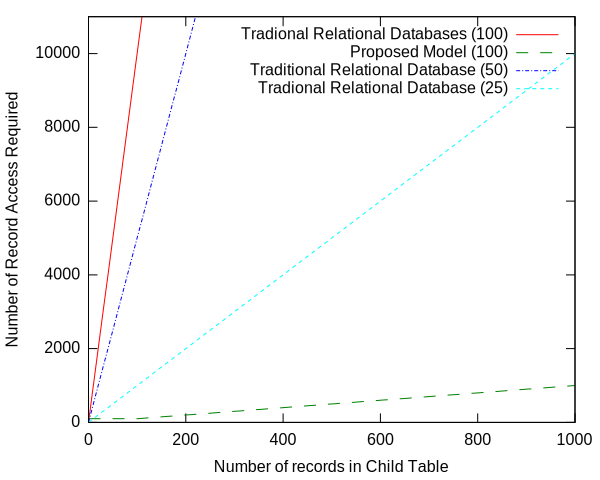
\includegraphics[width=\textwidth]{pics/time.pdf}
 \caption{Time Taken for Join Query}
 \label{fig:timeresult}
\end{figure}
A linear relation was observed to exist between the number of records and time taken for join query.
\subsection{Objectives Achieved}
As mentioned previously, we had particular objectives to achieve during the course of this project. We have been able to achieve most of those objectives as mentioned in the following section.
\subsubsection{Relational Model vs Graph Model}
We were able to get more insights about the graph based storage and the storage model in relational database after implementation of the proposed model. We observed the following :
\begin{itemize}
 \item The proposed graph database has lot of overhead due to pointers and implicit indexing. The amount of meta-data required to be stored with graph model might also be more than the meta-data stored with traditional relational databases. If the actual data do not have sufficient redundancy then the proposed model performs poorly.
 \item If there is a lot of redundant data or the size of the actual value is only a small fraction of the maximum allowed size for the corresponding attribute then the overhead in graph model is less corresponding to the gain in terms of storage.
 \item Theoretically the time bound for any type of query is same in the proposed model and is less than or equal to that of the traditional relational database storage. This means that the proposed model is much faster in terms of time taken. Our model is better in performing the Inner Join Queries which have a theoretical upper bound of $\mathcal{O}(max(m, n))$ where, $m, n$ is the number of records in the two relations being joined. It can be further reduced to $\mathcal{O}(min(m,n))$ if the query algorithm is most optimal.
 \item The growth stage of the database i.e., when the number of records is steadily rising in database the graph based storage might seem to be slower despite same time complexity owing to large constant. However, once the database is stable and select queries become the most frequent one, then proposed graph model performs much faster. Also the proposed model requires periodic deletion of invalid (soft deleted) records.
\end{itemize}
\subsubsection{Relational Algebraic Operations}
Our proposed model is successfully able to represent any relational database. All the relational algebraic operations are supported by our model.
\begin{itemize}
 \item \textbf{Project} - The model that we propose handles projection very easily. Given a Tuple, to apply the Projection operation we go to it's Main node and only access those attributes that the projection operation demands.
 \item \textbf{Select} - The model proposed is able to handle the application of propositional formula. The performance of the select operation is dependent on the order in which the formula are applied along with the logical operators. Our model is able to handle the binary operation "=" very effectively due to the indexing option given to the user. In the worst case it performs the operation in $\mathcal{O}(n)$. Other logical operators like $ <, >, \leq, \geq, \neq$,  require $\mathcal{O}(n)$ for all cases.
 \item \textbf{Natural Join} - In the model proposed the Select operation can be implemented by using the links that connect the main nodes of two tables which are related to each other through foreign key relationship. This is done in O(N) where N varies between the size of the records of the two tables depending on the way the propositional formula is solved.
\end{itemize}


\chapter{Future Work}
There are various optimizations and techniques that couldn't be implemented in the current version of source code owing to shortage of time. In this chapter we will discuss the major future works that can be undertaken with regard to this project.
\section{Parallel Execution of Queries}
Various Queries especially - Select and Join queries are read only. Moreover in our model, queries like these typically access data belonging to different relations. As such, these queries can easily be executed in parallel fashion. In current implementation we often determine multiple set of results and then take Intersection (AND operator) or Union (OR operator) to obtain the final result. During Intersection we choose the size of minimum set and iterate over it to check if it belongs to all the other sets. Such operations are embarrassingly parallel. We can fetch different set of results on different threads. \par
We can use pthreads or openmp for the said purpose. We can use General Purpose Graphic Processing Unit(GPGPU) Libraries like Cuda or OpenCL to create large number of threads which may perform better.
\section{Hybrid Adapting Model}
There is obviously no solution optimized for each situation. Relational Database might still be better than our proposed model in many cases. For example, if most of the records in a relation are unique, then the overhead of storing pointers is more than the gain due to redundancy in our proposed model. Again, if most of the queries performed do not require index lookups and are purely aggregate in nature pure graph databases might perform much better than the proposed model as well as relational databases. As such the most optimized method seems to be the one where an appropriate storage module is adapted based on the frequency of the queries being executed on the system. \par
When database is newly created and number of records are growing at a fast rate relational databases should be used. When the system is saturated with data and uses the database only for reading / updating, the proposed model might be optimal. The switch-over between the models will be determined by a number of parameters like database design, storage overhead, data redundancy, query etc. One can also use Machine Learning methods to train the system to select best model based on the type of most frequent queries and the corresponding query plan.
\section{Optimal Data Structures}
\subsection{Nodes}
Currently Attribute Nodes and Main Nodes are stored as a Linked List in corresponding table or domain. Main Nodes are stored as a doubly linked list, while attribute node is a singly linked list. However, this might not be the most optimized data structures for every situation. For Example, if the frequency of delete operation is low then an extra reverse pointers in doubly linked list node (main node) is an overhead in the long-run. If the number of new attribute nodes inserted in the domain falls over time i.e., new values are rare and all new records uses existing values, then a sorted list of attribute nodes will be more efficient as aggregate queries can be performed much faster. All the choices of data structures to be used for internal implementation mostly depends on the type of queries performed. The system can be tuned to perform only a particular type of query optimally while still supporting other types of queries.
\subsection{Indexing}
The data structure used for indexing in the current implementation is trie - which is known for its storage overheads. Moreover, all the data types are stored as strings in the attribute node - including the integers and floating point values. The performance can be drastically improved in terms of both storage overheads and query execution time if all data is stored in its native format and an optimal indexing is used for each data type. For Example, any Balanced Binary Search Tree will perform much better than trie for looking up integral and floating point values. They even have less storage overhead. However, handling different data structures for different data types might be tedious task for the developers. The foremost optimization would be the use of compressed trie data structure which improves the storage overhead of the existing normal trie. \\ \par
The switch over between different data structures has its own overhead and might require inputs from DB Administrator. Query service might also be unavailable during the switch over.
\subsection{Constraints}
The model to handle foreign-key can also be adapted to suit a particular application. However, this might be one of the most difficult adaption to implement as the method to handle foreign-keys is tightly coupled with the storage model. If the type of queries are known before the database is created, we might still be able to choose the best model.
\section{Query Optimization}
In current implementation, all the select and join queries are executed in a generic fashion. However it is very intuitive to observe that using a bit of estimation, statistics and relational algebra we can re-arrange the expressions in the where clause such that we take least time to execute the query. There should be a query plan for each query which specifies the best route to be taken while traversing the graph nodes and edges. A lot of research has been done in this area already and an existing query optimizer from relational database can be used for our proposed storage model.

\pagebreak
\bibliographystyle{ieeetr}
\bibliography{biblio}
\addcontentsline{toc}{chapter}{Bibliography}
%\addcontentsline{toc}{chapter}{Appendix Paper 1}
%\includepdf[pages={1-9}]{paper1.pdf}
%\addcontentsline{toc}{chapter}{Appendix Paper 2}
%\includepdf[pages={1-6}]{paper2.pdf}
\end{document}